\documentclass{article}
\usepackage{graphicx}
\usepackage[position=top]{subfig}
\usepackage[left=1in,right=1in,top=1in,bottom=1in]{geometry}
 \usepackage{pxfonts}


 \newcommand{\familiarity}{2}



\begin{document}

\title{Supporting Materials for \textit{Category-based and location-based volitional covert attention affect
memory at different timescales}}

\author{Kirsten Ziman$^1, 2$,
Madeline R. Lee$^1$,
Alejandro R. Martinez$^1$,\\
Ethan D. Adner$^1$,
and
Jeremy R. Manning\textsuperscript{$1, \dagger$}\\[0.1in]$^1$Dartmouth College\\
$^2$Princeton University\\
\textsuperscript{$\dagger$}Address correspondence to jeremy.r.manning@dartmouth.edu}


%\begin{titlepage}
  \maketitle
%\end{titlepage}

  \renewcommand{\thefigure}{S\arabic{figure}}


  \begin{figure*}[tp]
	\centering
	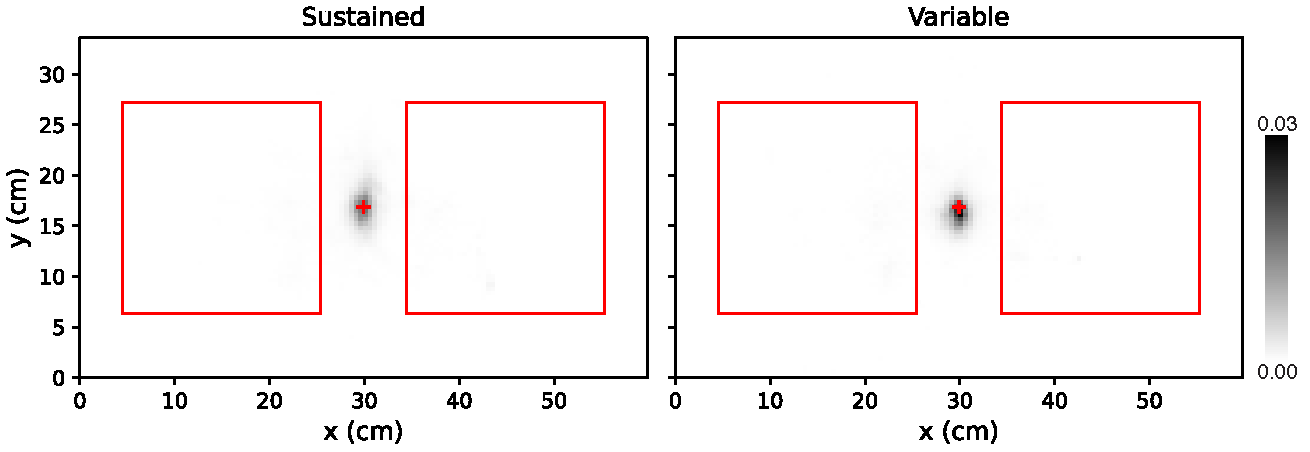
\includegraphics[width=1\textwidth]{figs/gaze_locations}
  
 \caption{\textbf{Gaze location histograms.} We divided the experimental
 display into 120 horizontal bins and 78 vertical bins, each comprising a
 roughly 0.5~cm square. The panels display the average proportions of time
 (throughout the duration of the experiment) participants spend looking at each
 location. The left panel displays data from participants in the sustained
 attention condition and the right panel displays data from participants in the
 variable attention condition. In both panels, the locations of the central
 fixation cross (red $+$) and composite images (red-outlined squares) are
 indicated.}
  
  \label{fig:gaze-histograms}
  \end{figure*}

  \begin{figure*}[tp]
	\centering
	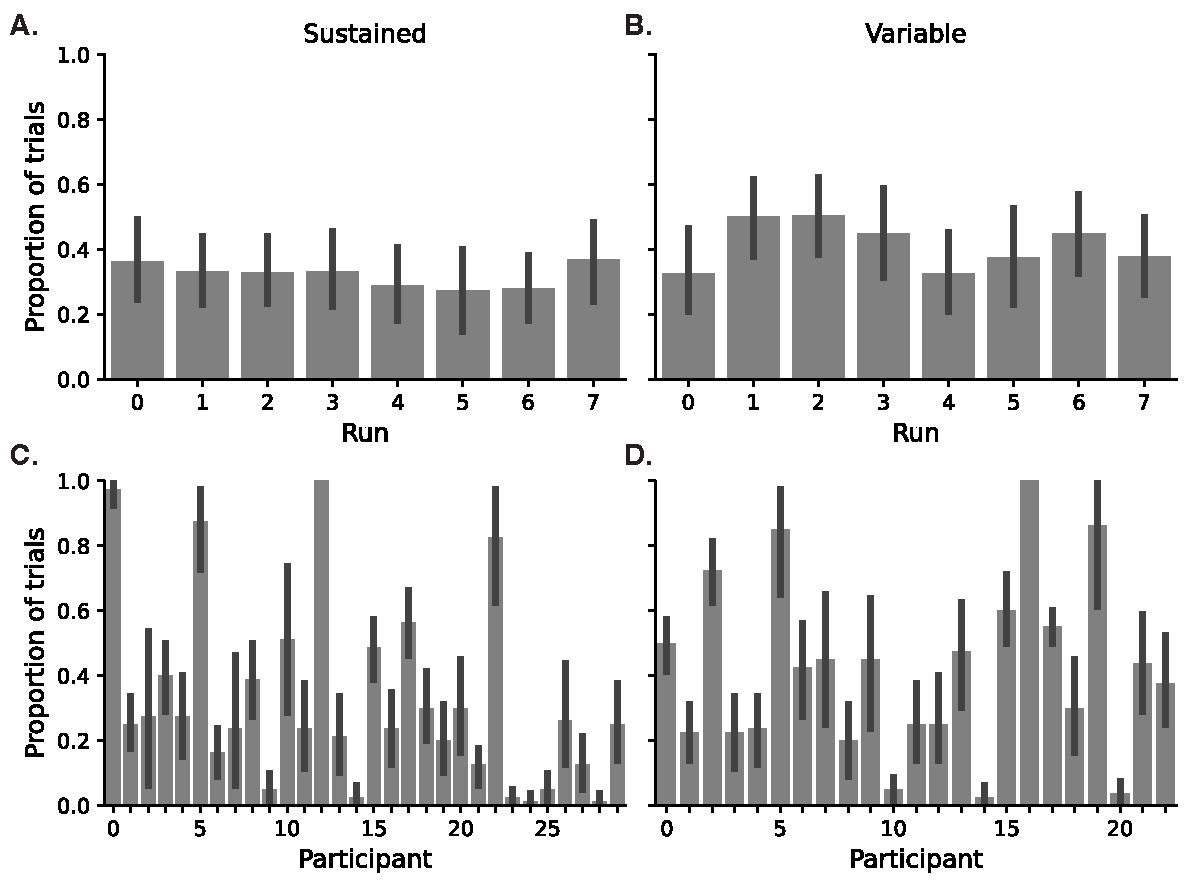
\includegraphics[width=1\textwidth]{figs/gaze_intersections}
  
\caption{\textbf{Proportions of excluded trials.} We excluded from our analyses
any images from trials where the participant's gaze touched on any part of the
attended composite image (attended-side red squares in
Fig.~\ref{fig:gaze-histograms}). \textbf{A--B. Proportions of excluded trials,
by run.} Across both experimental conditions (left: sustained attention; right:
variable attention), the bars display the average proportions of presentations
from each run where participants looked at any part of the attended composite
image, for any non-zero duration. Error bars denote across-participant
bootstrap-estimated 95\% confidence intervals. \textbf{C--D. Proportions of
excluded trials, by participant.} Across both experimental conditions (left:
sustained attention; right: variable attention), the bars display the average
proportions of presentations across different runs where the given
pariticapants looked at any part of the attended composite image, for any
non-zero duration. Error bars denote across-run bootstrap-estimated 95\%
confidence intervals.}
  
  \label{fig:intersections}
  \end{figure*}

  \label{fig:gaze-histograms}
\end{figure*}

\begin{figure*}[tp]
  \centering
  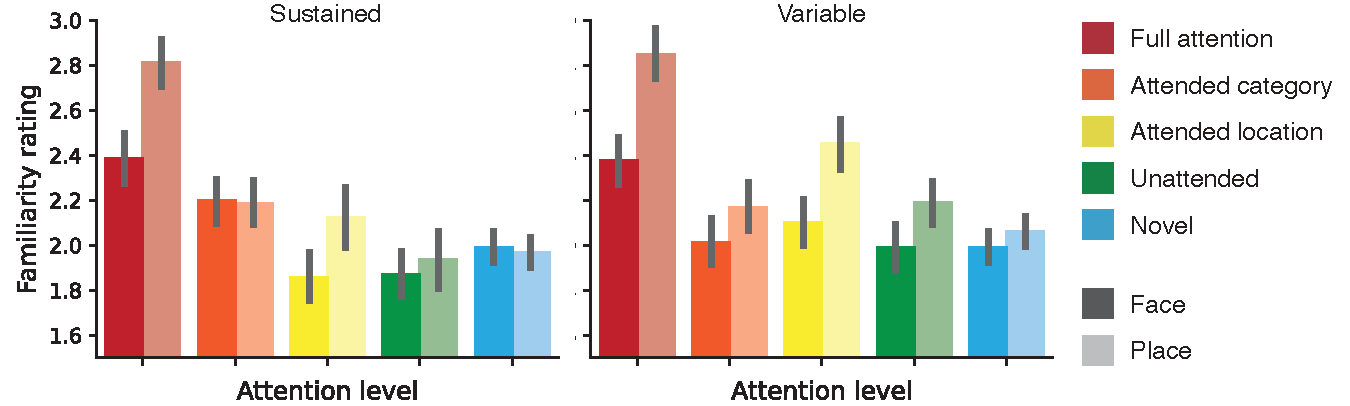
\includegraphics[width=1\textwidth]{figs/familiarity_by_attention_level and_category}

\caption{\textbf{Familiarity by attention level and stimulus category.} The
bars display the average familiarity ratings participants gave to images from
the same category and location as the attention cue (fully attended), the same
category (but opposite location) as the attention cue (attended category), the
same location (but opposite category) as the attention cue (attended location),
the opposite category and location as the attention cue (unattended), or novel
images. Each family of bars is further sub-divided according to whether the
rated stimulus was a face (darker shading) or a place (lighter shading) image.
The left panel displays familiarity ratings from the sustained attention
condition and the right panel displays familiarity ratings from the variable
attention condition. All error bars denote across-participant
bootstrap-estimated 95\% confidence intervals. Also see Figure~\familiarity~in
the main text.}

\label{fig:ratings-by-category}
\end{figure*}






\end{document}
